% Copyright 2016 - 2017 Bas van Meerten and Wouter Franssen
%
%This file is part of ssNake.
%
%ssNake is free software: you can redistribute it and/or modify
%it under the terms of the GNU General Public License as published by
%the Free Software Foundation, either version 3 of the License, or
%(at your option) any later version.
%
%ssNake is distributed in the hope that it will be useful,
%but WITHOUT ANY WARRANTY; without even the implied warranty of
%MERCHANTABILITY or FITNESS FOR A PARTICULAR PURPOSE.  See the
%GNU General Public License for more details.
%
%You should have received a copy of the GNU General Public License
%along with ssNake. If not, see <http://www.gnu.org/licenses/>.

\documentclass[11pt,a4paper]{article}
\include{DeStijl}

\usepackage[bitstream-charter]{mathdesign}
\usepackage[T1]{fontenc}
\usepackage[protrusion=true,expansion,tracking=true]{microtype}
\pgfplotsset{compat=1.7,/pgf/number format/1000 sep={}, axis lines*=left,axis line style={gray},every outer x axis line/.append style={-stealth'},every outer y axis line/.append style={-stealth'},tick label style={font=\small},label style={font=\small},legend style={font=\footnotesize}}
\usepackage{colortbl}
\usetikzlibrary{calc}

%Set section font
\usepackage{sectsty}
\allsectionsfont{\color{black!70}\fontfamily{SourceSansPro-LF}\selectfont}
%--------------------


%Set toc fonts
\usepackage{tocloft}
%\renewcommand\cftchapfont{\fontfamily{SourceSansPro-LF}\bfseries}
\renewcommand\cfttoctitlefont{\color{black!70}\Huge\fontfamily{SourceSansPro-LF}\bfseries}
\renewcommand\cftsecfont{\fontfamily{SourceSansPro-LF}\selectfont}
%\renewcommand\cftchappagefont{\fontfamily{SourceSansPro-LF}\bfseries}
\renewcommand\cftsecpagefont{\fontfamily{SourceSansPro-LF}\selectfont}
\renewcommand\cftsubsecfont{\fontfamily{SourceSansPro-LF}\selectfont}
\renewcommand\cftsubsecpagefont{\fontfamily{SourceSansPro-LF}\selectfont}
%--------------------

%Define header/foot
\usepackage{fancyhdr}
\pagestyle{fancy}
\fancyhead[LE,RO]{\fontfamily{SourceSansPro-LF}\selectfont \thepage}
\fancyhead[LO,RE]{\fontfamily{SourceSansPro-LF}\selectfont \leftmark}
\fancyfoot[C]{}
%--------------------

%remove page number from first chapter page
\makeatletter
\let\ps@plain\ps@empty
\makeatother
%----------------------
\usepackage{blindtext, color}
\definecolor{gray75}{gray}{0.75}
\newcommand{\hsp}{\hspace{20pt}}



\usepackage[hidelinks,colorlinks,allcolors=black, pdftitle={Nutation},pdfauthor={W.M.J.\ Franssen}]{hyperref}

\interfootnotelinepenalty=10000 %prevents splitting of footnote over multiple pages
\linespread{1.2}

%\usepgfplotslibrary{external}%creates all external tikz images that are included.
%\tikzexternalize[shell escape=-enable-write18]%activate externalization
%\tikzsetexternalprefix{GeneratedFigures/}
%\tikzset{external/force remake} %Enable forced remake

\title{\color{black}\fontfamily{SourceSansPro-LF}\bfseries Nutation data analysis using ssNake}
\date{\color{black}\fontfamily{SourceSansPro-LF}\bfseries \today}


\begin{document}
\input{PulseSeq.tex}
%\newgeometry{left=72pt,right=72pt,top=95pt,bottom=95pt,footnotesep=0.5cm}
\microtypesetup{protrusion=true} % enables protrusion

\maketitle

\section{Introduction}
This tutorial will explain how a standard nutation experiment can be processed in ssNake.
The tutorial delivered with the ssNake program is considered as prior knowledge.
If you have not yet studied this, please do so before continuing with this example.

A nutation experiment is a series of single pulse NMR experiment with an increasing pulse length (see Figure~\ref{fig:pulsseq}.
In this way, the modulation of the signal during the pulse can be studied.
When the RF field strength is large, the effects of chemical shift can be ignored during the pulse, which leads to a sine modulation of the signal intensity with a frequency $\nu_1$: the nutation frequency.
Knowledge of the nutation frequency (i.e. the RF field strength) can be used for setting up decoupling sequences, cross-polarization, and so on.

\begin{center}
\begin{tikzpicture}[scale=0.8]
\coordinate (Position) at (0,0); %Start at this point. For additional nucleus start at a lower point.
%\Nucleus{$^{139}$La}
\ExPulse[$\phi_1$][$t_1$]{\arrowheigth}
\FID[][$t_2$]{}
\end{tikzpicture}
\captionof{figure}{Pulse sequence of a single pulse nutation experiment.}\label{fig:pulsseq}
\end{center}




\section{Used data}
For this example, we will use a Varian data set recorded on a 14.1~T spectrometer.
The sample was a saturated solution of KMnO$_4$ in water, and the $^{55}$Mn signal was recorded.
In this data set, an array of experiment was performed, with the pulse length starting at 6~$\muup$s, and increasing with 6~$\muup$s with a total of 128 experiments.
For the analysis described here, it is required that the step size and initial value are equal.

\section{Processing}
\begin{itemize}
\item Open the data file by using File $\longrightarrow$ Open.
\item Zero fill the data to 4k points (4096 points) by using Matrix $\longrightarrow$ Sizing, and filling in the value in the Size box.
\item Fourier transform using the `Fourier' button in the bottom frame.
\end{itemize}
This shows us the spectrum of the first experiment (with a 6~$\muup$s pulse width).
\begin{itemize}
\item Phase this spectrum to obtain a nice absorption lineshape.
\end{itemize}
This results in the following figure:

\begin{center}
\includegraphics[width=0.8\linewidth]{Figs/Fig1.png}
%\captionof{figure}{Pulse sequence of a single puls enutation experiment.}\label{fig:fig1}
\end{center}


Now we can view the other experiments by increasing the value of the D1 box in the side frame.
Note that we want to continue to view the D2 dimension, and therefore keep the bullet next to D2 as the active dimension.

Now we would like to examine the change of the peak height along the D1 dimension.
We therefore need to obtain the position of the peak (in data points).
Click the `get position' button in the bottom frame, and select the top of the peak (zoom in for accurate).
This should report an x-position of approximately 2045.
To view this trace along D1, copy this value into the D2 box, and press press enter.
This results in the following Figure, which shows a sine oscillation as a function of pulse width:
\begin{center}
\includegraphics[width=0.8\linewidth]{Figs/Fig2.png}
\end{center}


\begin{itemize}
\item Zero fill along this D1 by using Matrix $\longrightarrow$ Sizing and use 1024 points.
\item Right shift the data with 1 point by using Matrix $\longrightarrow$ Shift Data, and click the right arrow button once. 
\end{itemize}
This should result in a figure similar to:
\begin{center}
\includegraphics[width=0.8\linewidth]{Figs/Fig3.png}
\end{center}

The last step we performed was to add a datapoint in front (with a value of 0) and removing a data point at the end.
This shift is required to make our data start at time zero and since a pulse width of 0 should give no signal we can do this by shifting our data by one data point.
This way, we artificially made our oscillation start at $t=0$.
For this reason it is convenient to have an initial value which is equal to the step size.


\begin{itemize}
  \item Transform to a spectrum by clicking the `Fourier' button.
\item Phase with -90$^\circ$ to obtain the in-phase spectrum.
\item Clear the reference frequency (no reference is required) via Tools $\longrightarrow$ Reference $\longrightarrow$ Clear Current Reference.
\end{itemize}
We should now set the sweepwidth to the correct value, so we obtain a sensible axis.
In our case, the dwell time of the experiment is the stepsize of the pulse width: 6~$\muup$s.
We can therefore type in the sweepwidth box in the bottomframe: `1000/6e-6'.
`1/6e-6' is the sweepwidth in Hz, and the 1000 is required to convert to kHz.
Alternatively, `1/6e-3' could also be used.
This results in to the following Figure, which is the final spectrum.
It shows an (nearly) anti-symmetric spectrum with a peak at 50~kHz, so $\nu_1 = 50\;$kHz in this case.
\begin{center}
\includegraphics[width=0.8\linewidth]{Figs/Fig4.png}
\end{center}

\section{Alternatives}
\subsection{Integrate D2}
When having phased the first spectrum in D2, Matrix $\longrightarrow$ Region $\longrightarrow$ Integrate can be used to integrate the peak.
Use the tool by left clicking on the left and right of the peak and press OK.
Continue the steps described above, but notice that the old D2 dimension has now been removed, and only the D1 remains.
As there is only one dimension now, the dimension selector in the side frame has disappeared.
This results in the following Figure (after 41.5$^\circ$ 1st order phasing):
\begin{center}
\includegraphics[width=0.8\linewidth]{Figs/Fig5.png}
\end{center}
Note that looks quite different form the `normal' processed spectrum.
This probably means that the nutation frequency varies over the peak.
This is probably caused by shimming issues, which result in a correlation between the NMR frequency (D2) and nutation frequency (D1).



\subsection{Force symmetry}
Ideally, the nutation spectrum has inversion symmetry (the left is -1 times the right).
Sometimes it is convenient to force this.
This can be done by performing Tools $\longrightarrow$ Real (removing the imaginary part) before the Fourier transform in the D1 domain.

\subsection{Correct DC offset}
In some cases, the nutation signal does not decay to zero, but to some other value.
This will result in a peak at 0 Hz in the nutation spectrum.
This can be avoided by subtracting the average of the last part of the nutation time signal from the entire signal.
This can be done by using Tools $\longrightarrow$ Subtract Averages.
Ideally, this is done before the zero filling the D1 domain.

\subsection{2D nutation}
When following the method to obtain the nutation spectrum, the spectrum can also be viewed as a contour plot.
This can be done through Plot $\longrightarrow$ Contour.


\end{document}
